\newpage
\section{Game of Life ohne Kommunikation (Aufgabe 10)}

Aufgabe 10 baut auf den vorherigen Aufgaben auf. In dieser Aufgabe wird das
Game of Life auf der LED-Matrix implementiert.

\subsection{Aufbau der Software}

\inputminted[linenos,fontsize=\footnotesize]{c}{A10_Abgabe/iceduino_setup_gol/sw/programs/iceduino_game_of_life/main.c}

In der Main wird das Setup der LED-Matrix durchgeführt und anschließend in
einer Endlosschleife das Game of Life ausgeführt. Eine neue Runde kann durch
das Drücken eines Tasters (Taster Nr.~2) ausgelöst werden. 
Der Steuercomputer, welcher die Anweisungen an den Slave sendet, stellt den
Master dar. Der Slave ist der lokale Teilnehmer, welche die Anweisungen vom Master
empfängt und ausführt. 
Um die Funktionsfähigkeit des Game of Life zu testen, wird ein virtueller
Master implementiert, welcher die Anweisungen an den Slave sendet.
Dieser
Master sendet MMCP Pakete an den Slave. Folgende Anweisungen sind
implementiert:
\begin{itemize}

  \item \textbf{set Muster}: Empfängt das einzustellende Initialmuster vom Master.
  \item \textbf{NextGen}: Weist den Slave an, die nächste Generation zu berechnen und auf der LED-Matrix darzustellen.
  \item \textbf{receiveEdge}: Hinzugefügt um die Imitation der Kantenbedingungen zu implementieren. Empfängt die Kantenbedingungen vom Master. Diese werden in den Payload des MMCP Pakets übertragen.

\end{itemize}

Der Slave reagiert anhand der empfangenen Anweisung. Hierbei können derzeit 4
verschieden States auftreten. Diese sind:
\begin{itemize}
  \item \textbf{STATE RECEIVE GRID}: Der Slave wartet auf eine Anweisung vom Master.
  \item \textbf{STATE RECEIVE EDGE}: Der Slave empfängt die Kantenbedingungen vom Master und speichert diese in einem Array.
  \item \textbf{STATE NEXT GEN}: Der Slave berechnet die nächste Generation und stellt diese auf der LED-Matrix dar.
  \item \textbf{STATE IDLE}: Der Slave empfängt das neue Raster vom Master und speichert es in einem der beiden Arrays.
\end{itemize}

Receive Grid wird durch die set Muster Anweisung vom Master ausgelöst. Receive
Edge wird durch die receiveEdge Anweisung vom Master ausgelöst. Next Gen wird
durch die NextGen Anweisung vom Master ausgelöst. Idle stellt einen
Standardzustand dar, welcher fehlerhafte Auslösungen verhindern soll.

Dies kann im folgenden Slave Code nachvollzogen werden:
\inputminted[linenos,fontsize=\footnotesize, firstline=364,
  lastline=452]{c}{A10_Abgabe/iceduino_setup_gol/sw/lib/source/game_of_life.c}

Nachfolgend wird die Berechnung der nächsten Generation, welche 
im Slave Code im Zustand STATE NEXT GEN zu finden ist, beschrieben.

Zur Berechnung einer neuen Generation wird das aktuelle Raster mit den
Kanteninformationen zusammengefügt.
\inputminted[linenos,fontsize=\footnotesize, firstline=289,
  lastline=337]{c}{A10_Abgabe/iceduino_setup_gol/sw/lib/source/game_of_life.c}
Danach wird die Anzahl der Nachbarn für jede Zelle berechnet. Hierfür werden
zwei Hilfsfunktionen verwendet. count\_live\_neighbors zählt die benachbarten
lebenden Zellen. update\_cell\_state aktualisiert den Zustand der Zelle
basierend auf den Regeln des Game of Life.
\inputminted[linenos,fontsize=\footnotesize, firstline=220,
  lastline=286]{c}{A10_Abgabe/iceduino_setup_gol/sw/lib/source/game_of_life.c}

Die neue Generation wird in einem der beiden Arrays, grid1 oder grid2,
gespeichert. Das andere Array dient als Ausgangsarray für die Berechnung der
nächsten Generation. Anschließend wird das neue Raster mithilfe der
write\_grid\_to\_matrix Funktion auf die LED-Matrix übertragen.
\inputminted[linenos,fontsize=\footnotesize, firstline=161,
  lastline=176]{c}{A10_Abgabe/iceduino_setup_gol/sw/lib/source/game_of_life.c}

Danach wird das Array, welches die alte Generation enthält, zurückgesetzt.
\inputminted[linenos,fontsize=\footnotesize, firstline=187,
  lastline=192]{c}{A10_Abgabe/iceduino_setup_gol/sw/lib/source/game_of_life.c}

Der beschrieben Ablauf ist der Kern der Implementation des Game of Life auf der
LED-Matrix. Die Kommunikation zwischen Master und Slave wird derzeit nur im
Code simuliert, um die Funktionalität zu testen. In zukünftigen
Implementierungen kann die Kommunikation über UART erfolgen, um die Anweisungen
vom Master an den Slave zu übertragen.

\subsection{Masterimitation}
Der folgende Code zeigt die Masterimitation, welche die Anweisungen an den
Slave sendet.
\inputminted[linenos,fontsize=\footnotesize,
  firstline=456,
  lastline=503]{c}{A10_Abgabe/iceduino_setup_gol/sw/lib/source/game_of_life.c}
Zur Zusammensetzung eines MMCP Pakets wird die Funktion build\_mmcp\_frame
verwendet. Diese setzt die einzelnen Bytes des Pakets zusammen und speichert
sie im rx\_buffer. \inputminted[linenos,fontsize=\footnotesize,
  firstline=342,
  lastline=362]{c}{A10_Abgabe/iceduino_setup_gol/sw/lib/source/game_of_life.c}

Der Master sendet zuerst ein Initialmuster an den Slave. Danach werden die
Kantendaten gesendet. Anschließend wird, bei jedem Knopfdruck, die nächste
Generation berechnet und auf der LED-Matrix dargestellt.

Der Master schreibt direkt in den rx\_buffer, um die Anweisungen zu
übermitteln. Dies ist eine Imitation der Kommunikation zwischen Master und
Slave. Das erleichtert die zukünftige Implementation der Kommunikation über
UART.

\subsection{Speicherorganisation}

\inputminted[linenos,fontsize=\footnotesize, firstline=4, lastline=11]{c}{A10_Abgabe/iceduino_setup_gol/sw/programs/iceduino_game_of_life/main.c}

Es werden zwei Arrays, grid1 und grid2, mit jeweils einer Länge von 8 Elementen
angelegt. Beide stellen das vollständige LED\-Raster dar, da acht uint8\_t
Werte insgesamt 64 Bits ergeben. Diese werden zur Darstellung der LED-Matrix
immer abwechselnd verwendet. Dadurch wird die Berechnung der nächsten
Generation vereinfacht, da immer nur ein Array als Ausgangsarray verwendet wird
und das andere Array als Zielarray dient. Zusätzlich wird ein Array
extended\_grid angelegt, welches das erweiterte Raster darstellt. Dieses Array
ist vom Typ uint16\_t. Dies ist nötig, da bei zehn Feldern eine Anzahl von
10x10 = 100 Bits benötigt werden. Es werden nur die ersten zehn Werte einer
jeden Arrayzeile verwendet.

Zusätzlich werden rx\_buffer und tx\_buffer Arrays angelegt, welche die
empfangenen und zu sendenden MMCP Pakete speichern. Diese sind jeweils 16 Byte
groß.

Auf einzelne Zellen wird durch Bitshifting zugegriffen. Dies ermöglicht eine
schlanke Speichernutzung. Eine Beispielhafte Zuweisung einer Zelle ist in
folgendem Code dargestellt:
\begin{minted}{c}

grid1[3] = grid1[3] | (0x1 << 5);
    
\end{minted}

Hierbei wird die Zelle in der dritten Zeile und der fünften Spalte auf
"`lebendig"' gesetzt.

Um möglichst wenig Kopieroperationen durchzuführen, werden diese Arrays per
Referenz an die Funktionen übergeben. Dies führt zu einer effizienten
Speicherorganisation und reduziert die Laufzeit der Software.

Die folgenden Definitonen für unterschiedliche Muster werden, nach Bedarf, vom
Compiler zur Optimierung gelöscht.
\inputminted[linenos,fontsize=\footnotesize, firstline=4,
  lastline=156]{c}{A10_Abgabe/iceduino_setup_gol/sw/lib/source/game_of_life.c}

\subsection{Implementation des Octagons}

Die folgenden Bilder zeigen die korrekte Darstellung des Octagons auf der
LED-Matrix.

\begin{figure}[H]
  \centering
  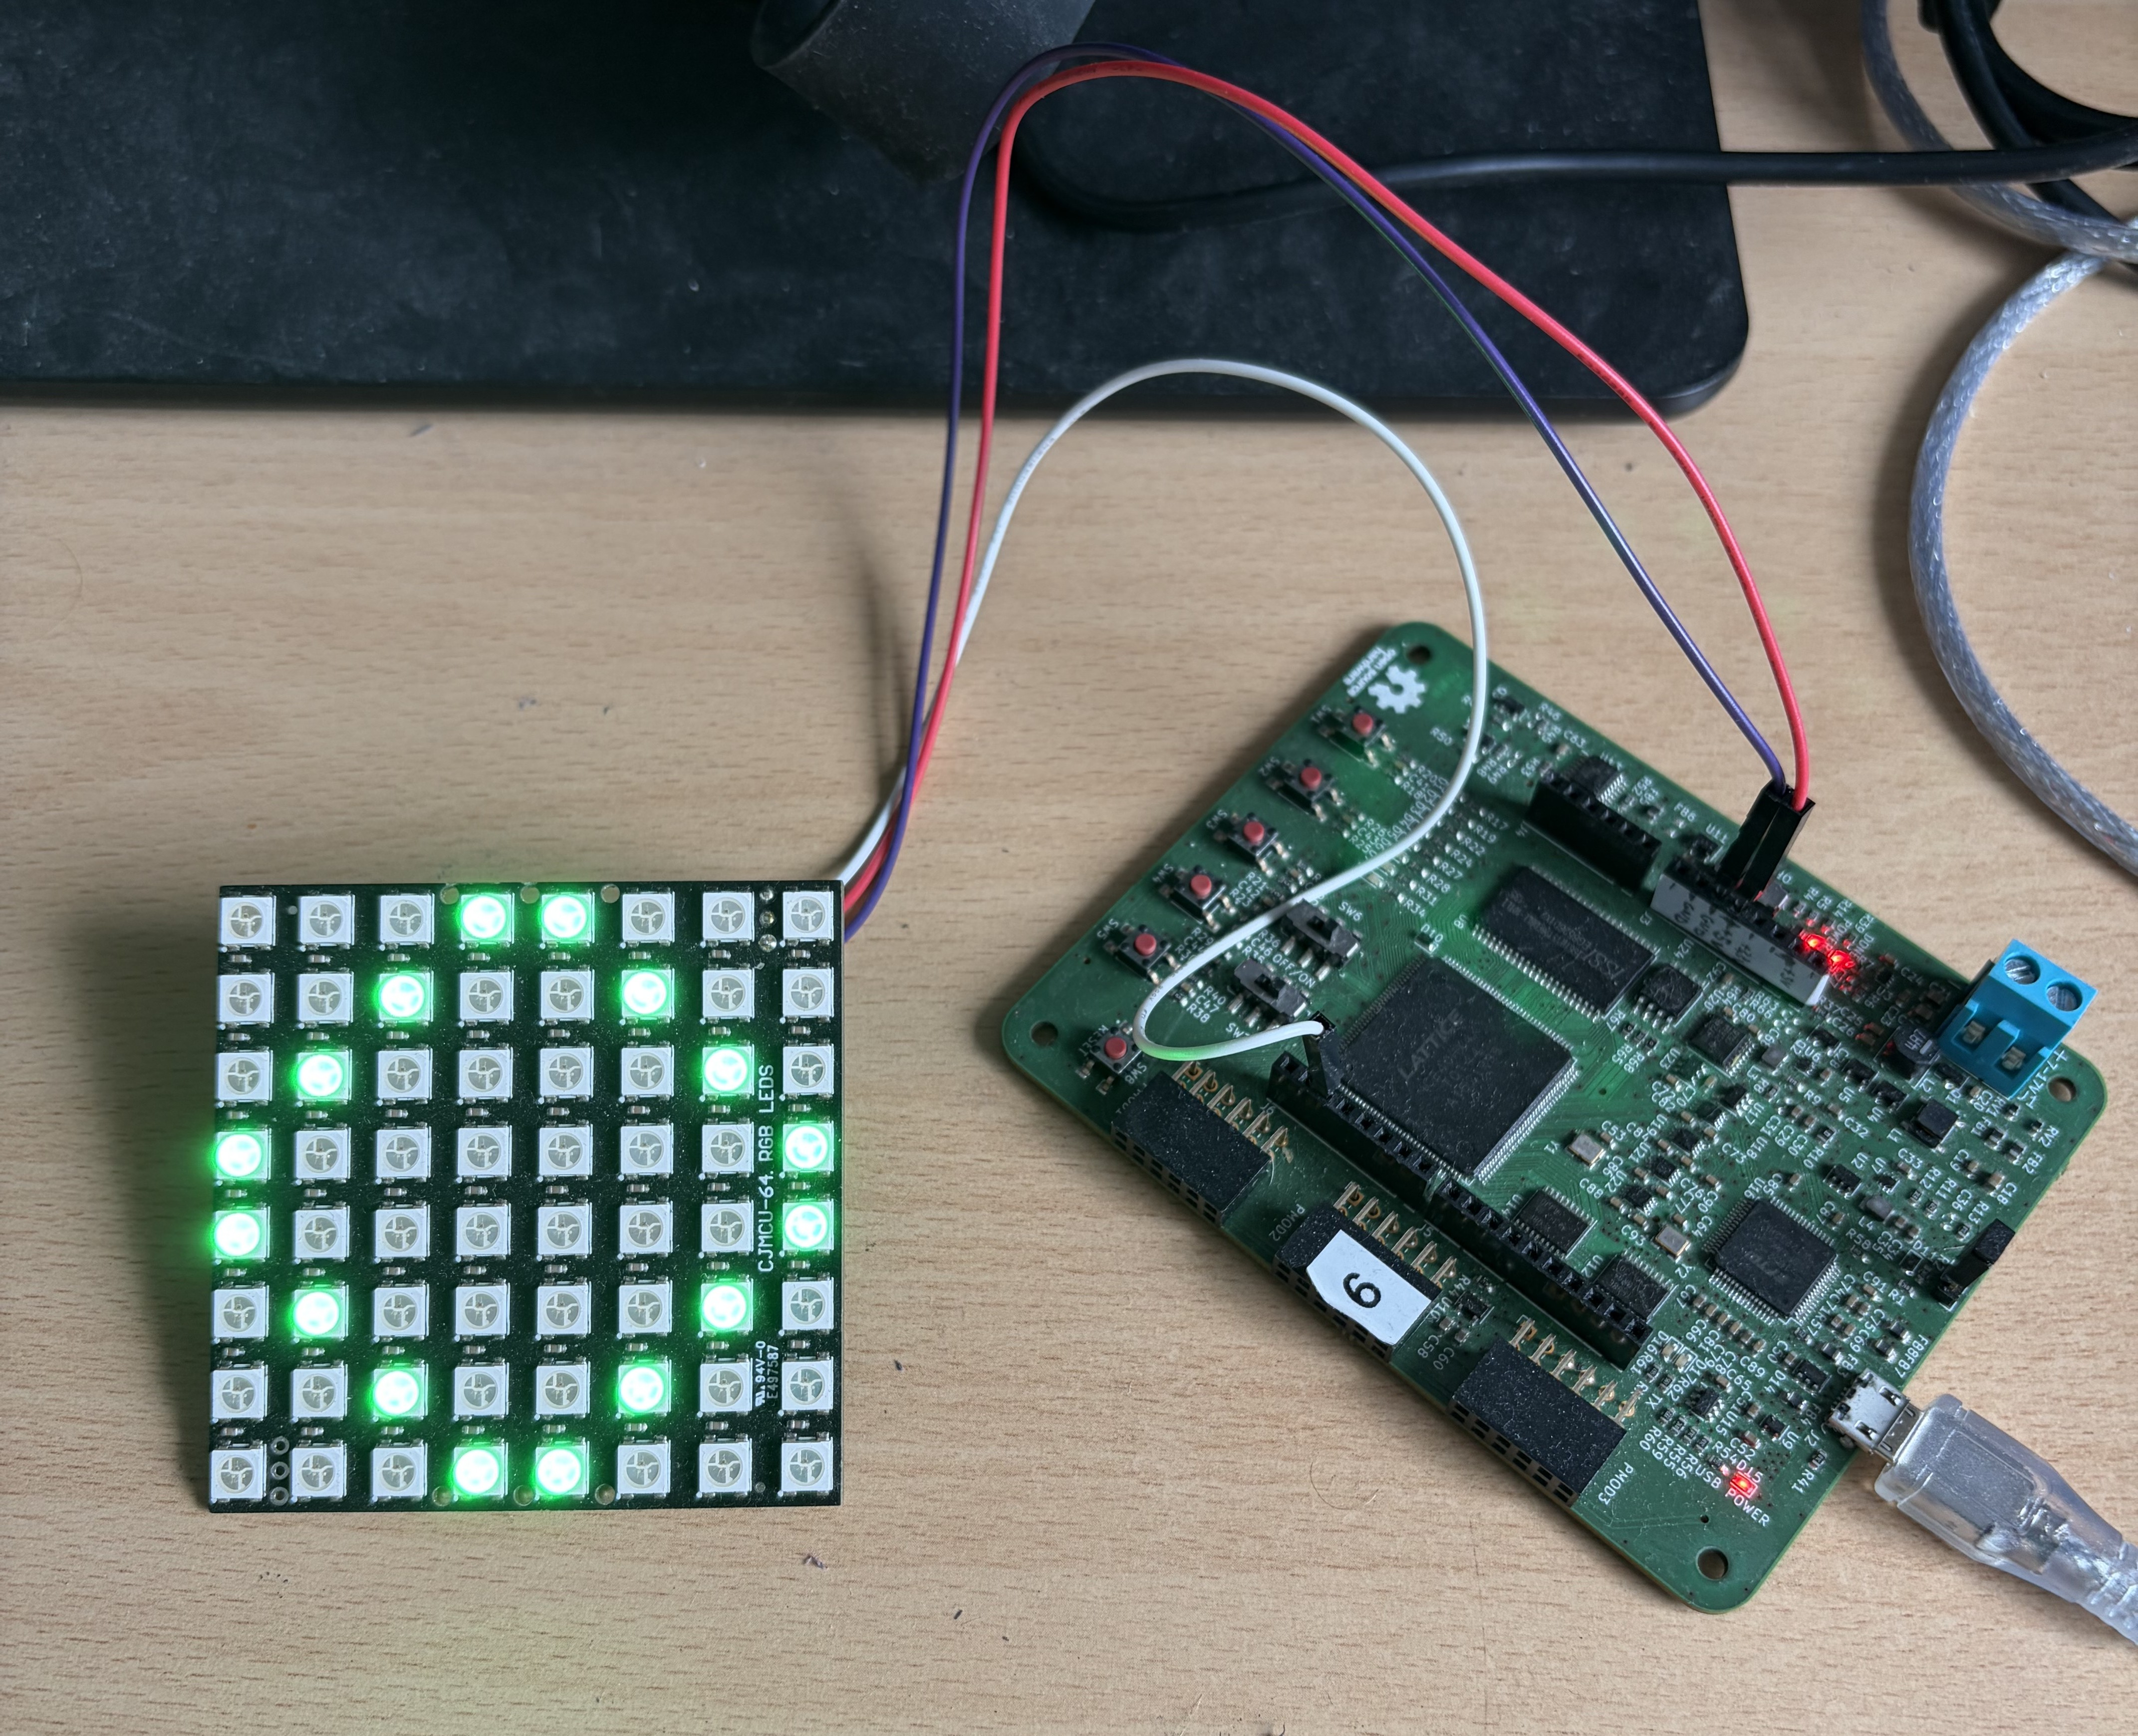
\includegraphics[width=\textwidth, angle=0]{A10_Abgabe/res/octagon_1.jpeg}
  \caption{Simulation des Octagon: Erste Generation}
  \label{fig:octagon_1}
\end{figure}

\begin{figure}[H]
  \centering
  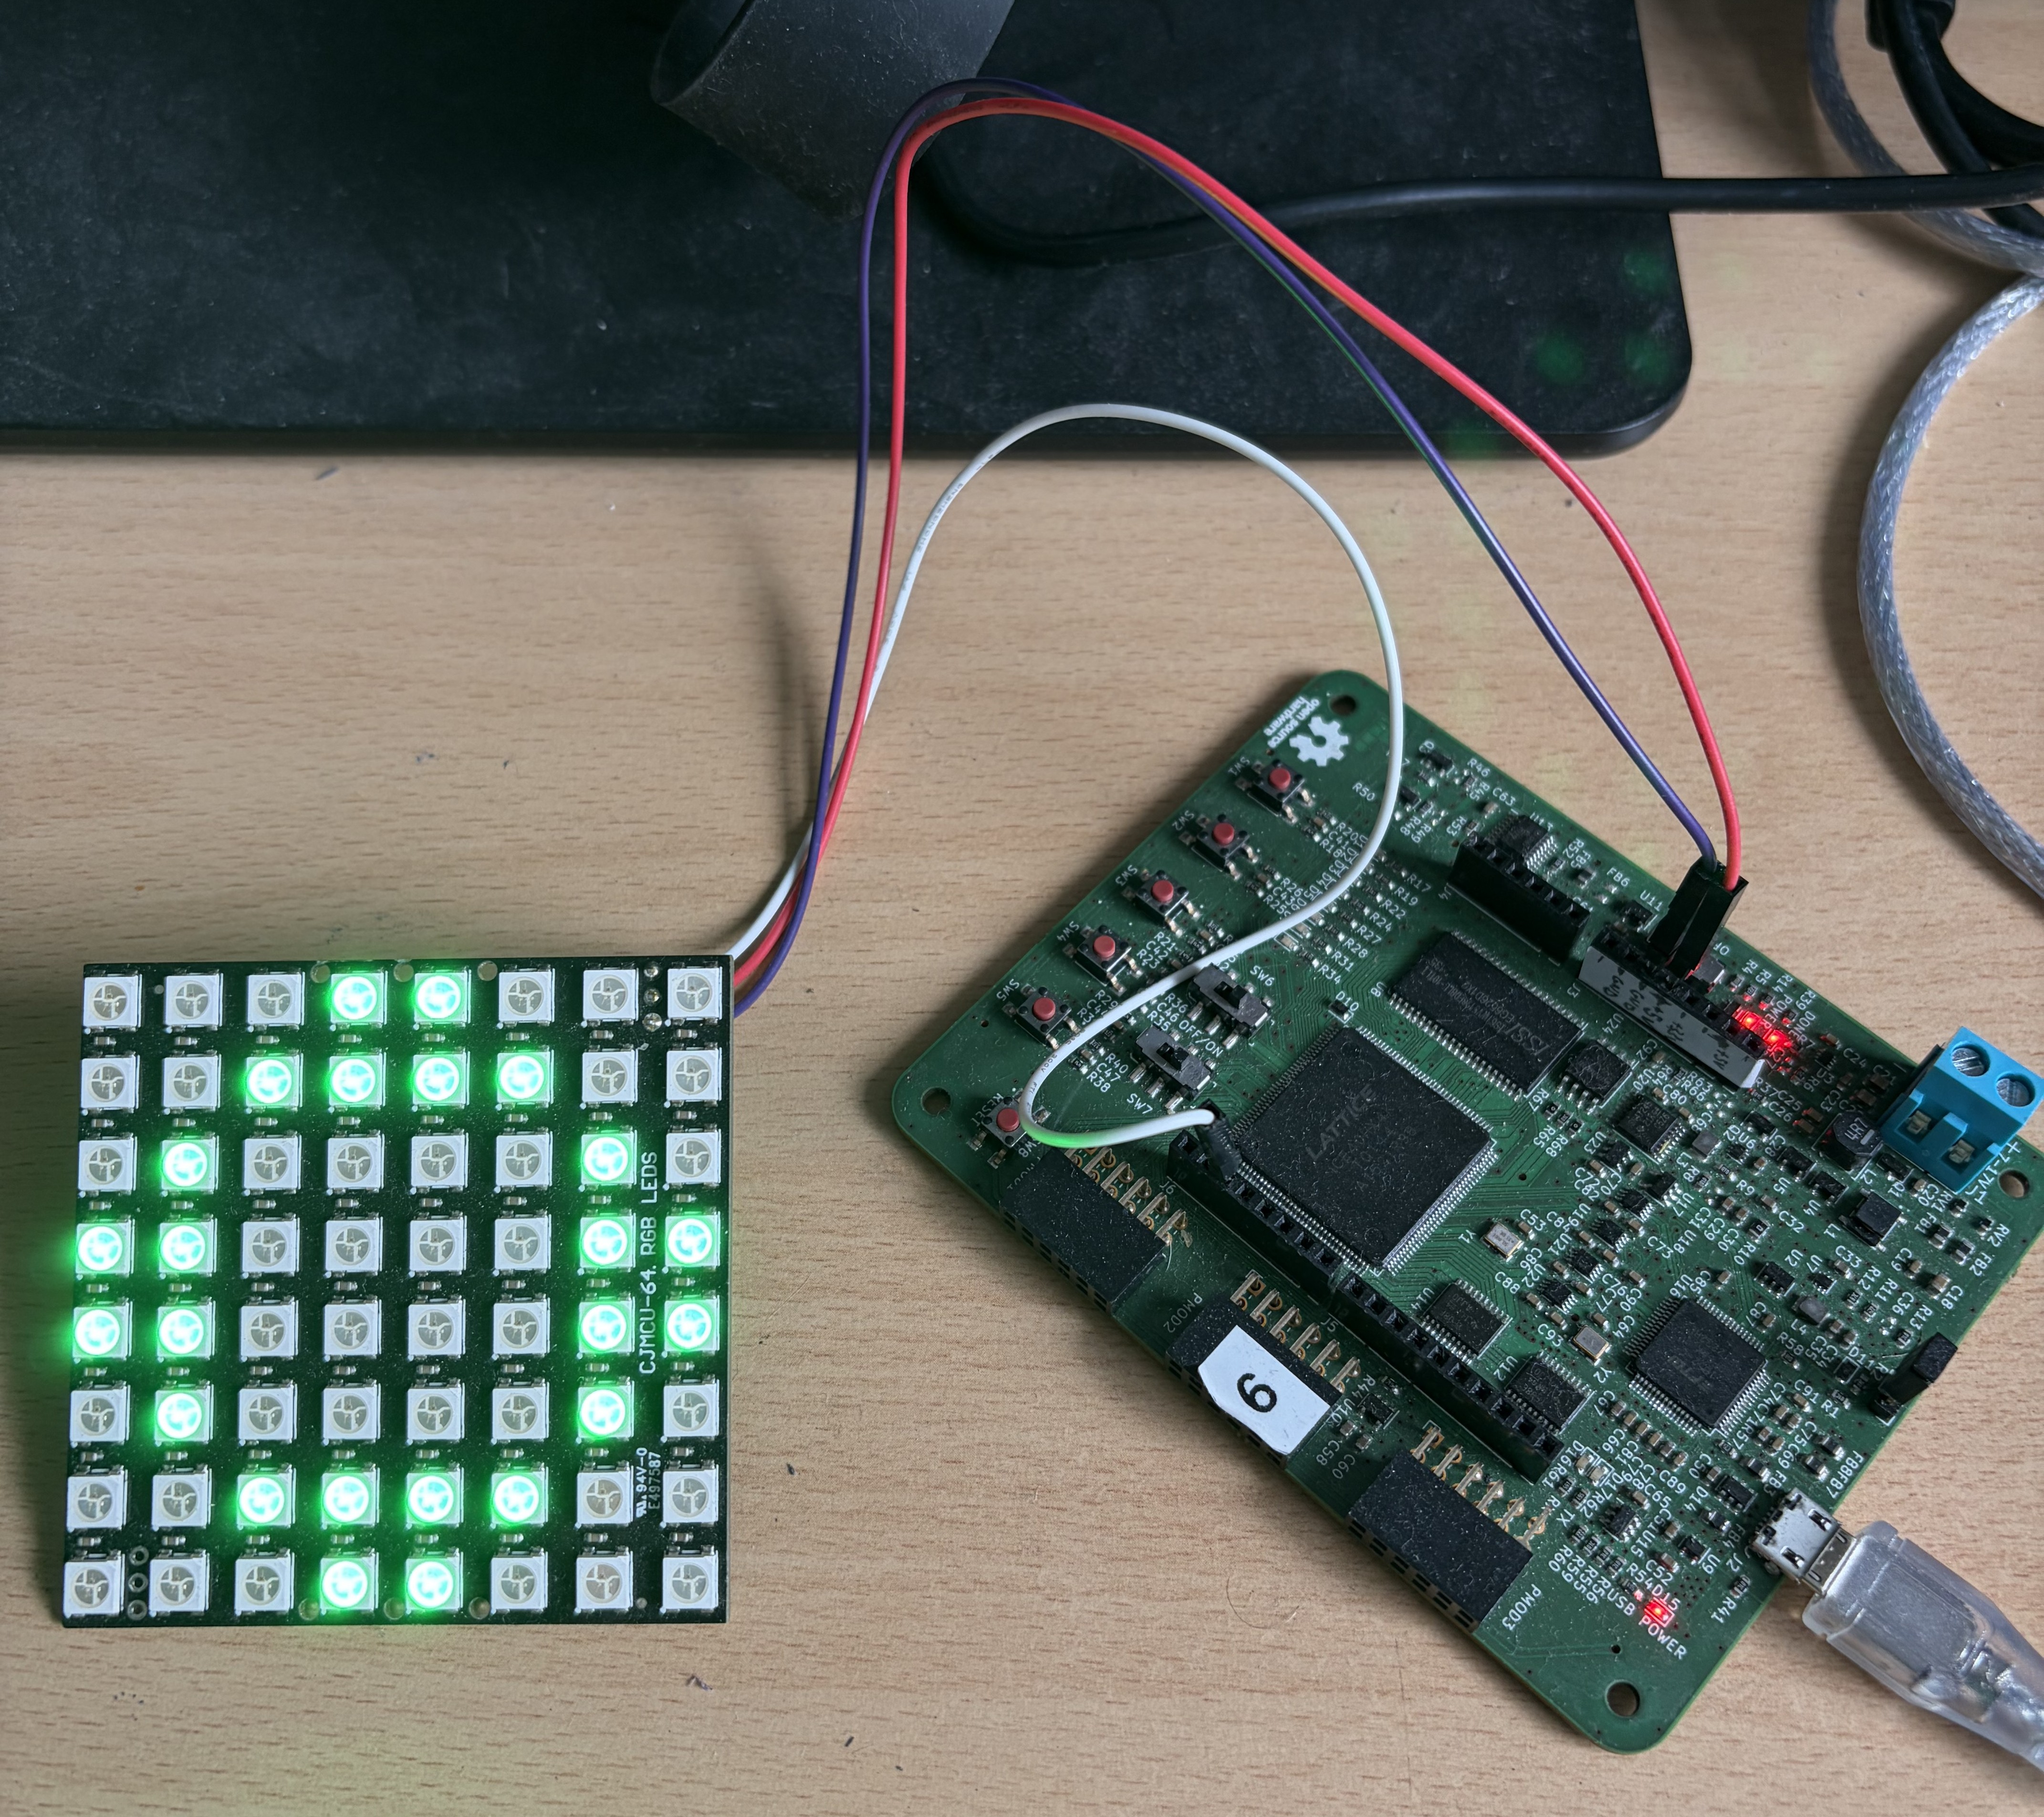
\includegraphics[width=\textwidth, angle=0]{A10_Abgabe/res/octagon_2.jpeg}
  \caption{Simulation des Octagon: Zweite Generation}
  \label{fig:octagon_2}
\end{figure}

\begin{figure}[H]
  \centering
  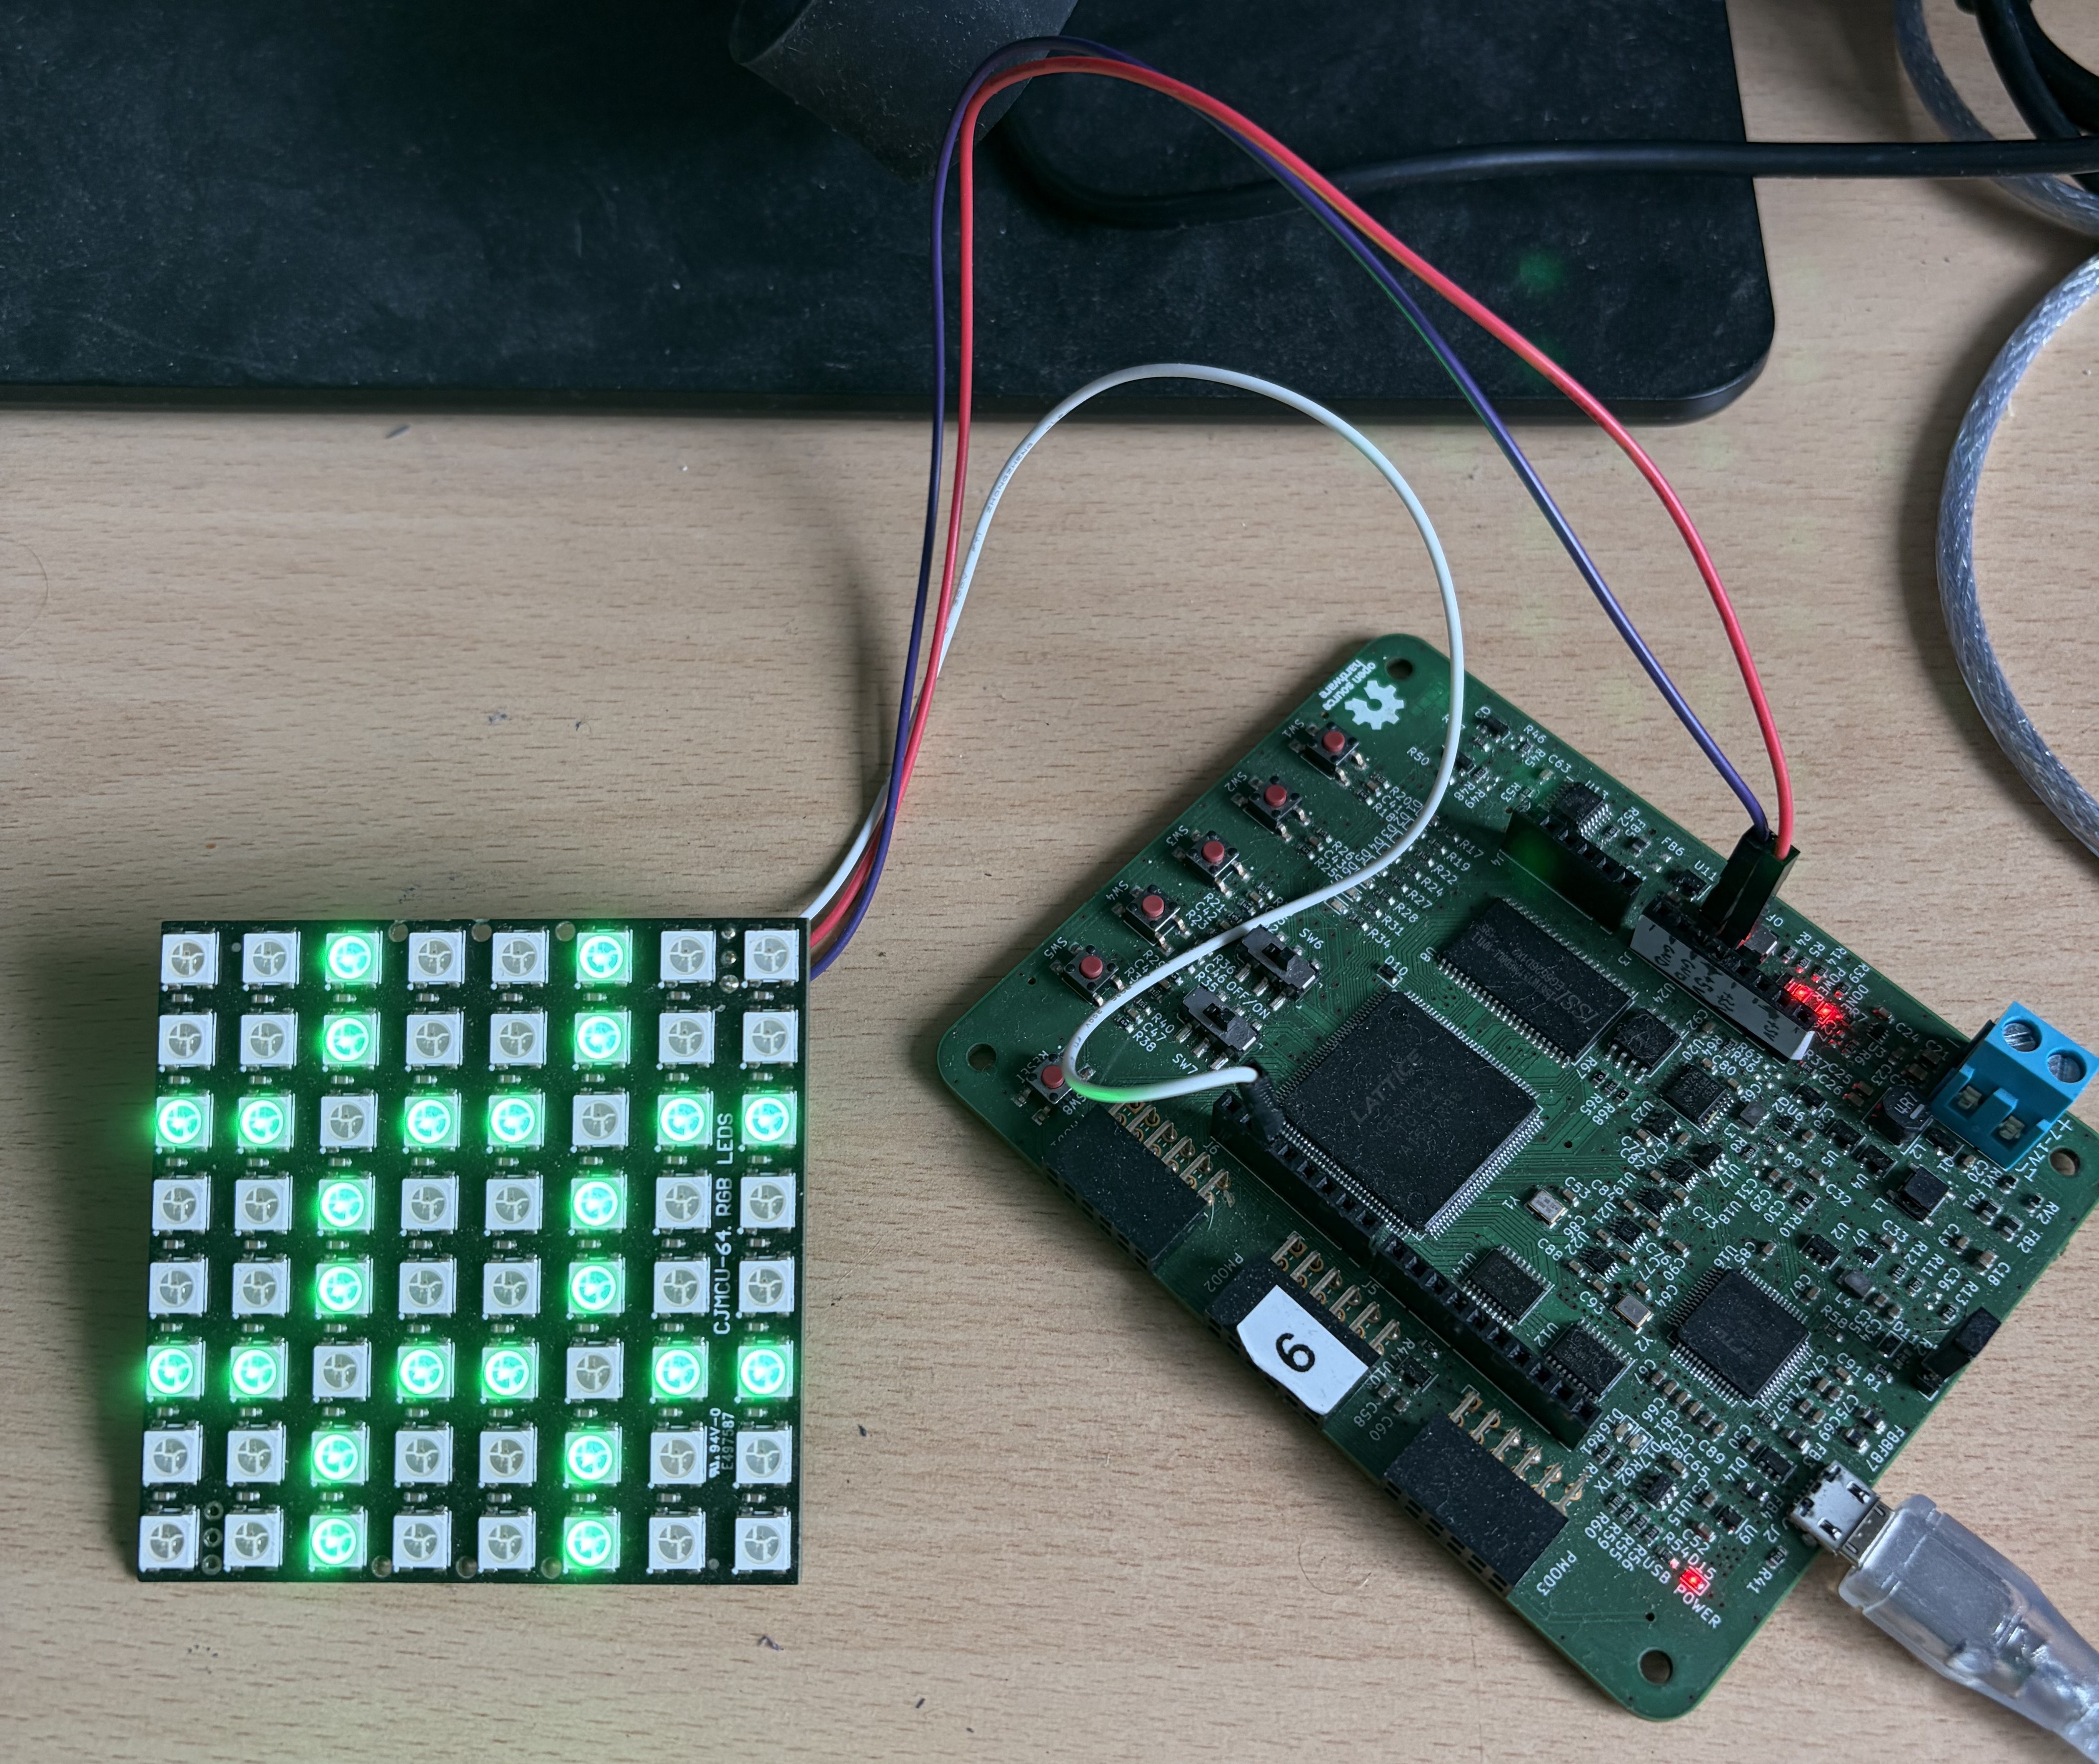
\includegraphics[width=\textwidth, angle=0]{A10_Abgabe/res/octagon_3.jpeg}
  \caption{Simulation des Octagon: Dritte Generation}
  \label{fig:octagon_3}
\end{figure}

\begin{figure}[H]
  \centering
  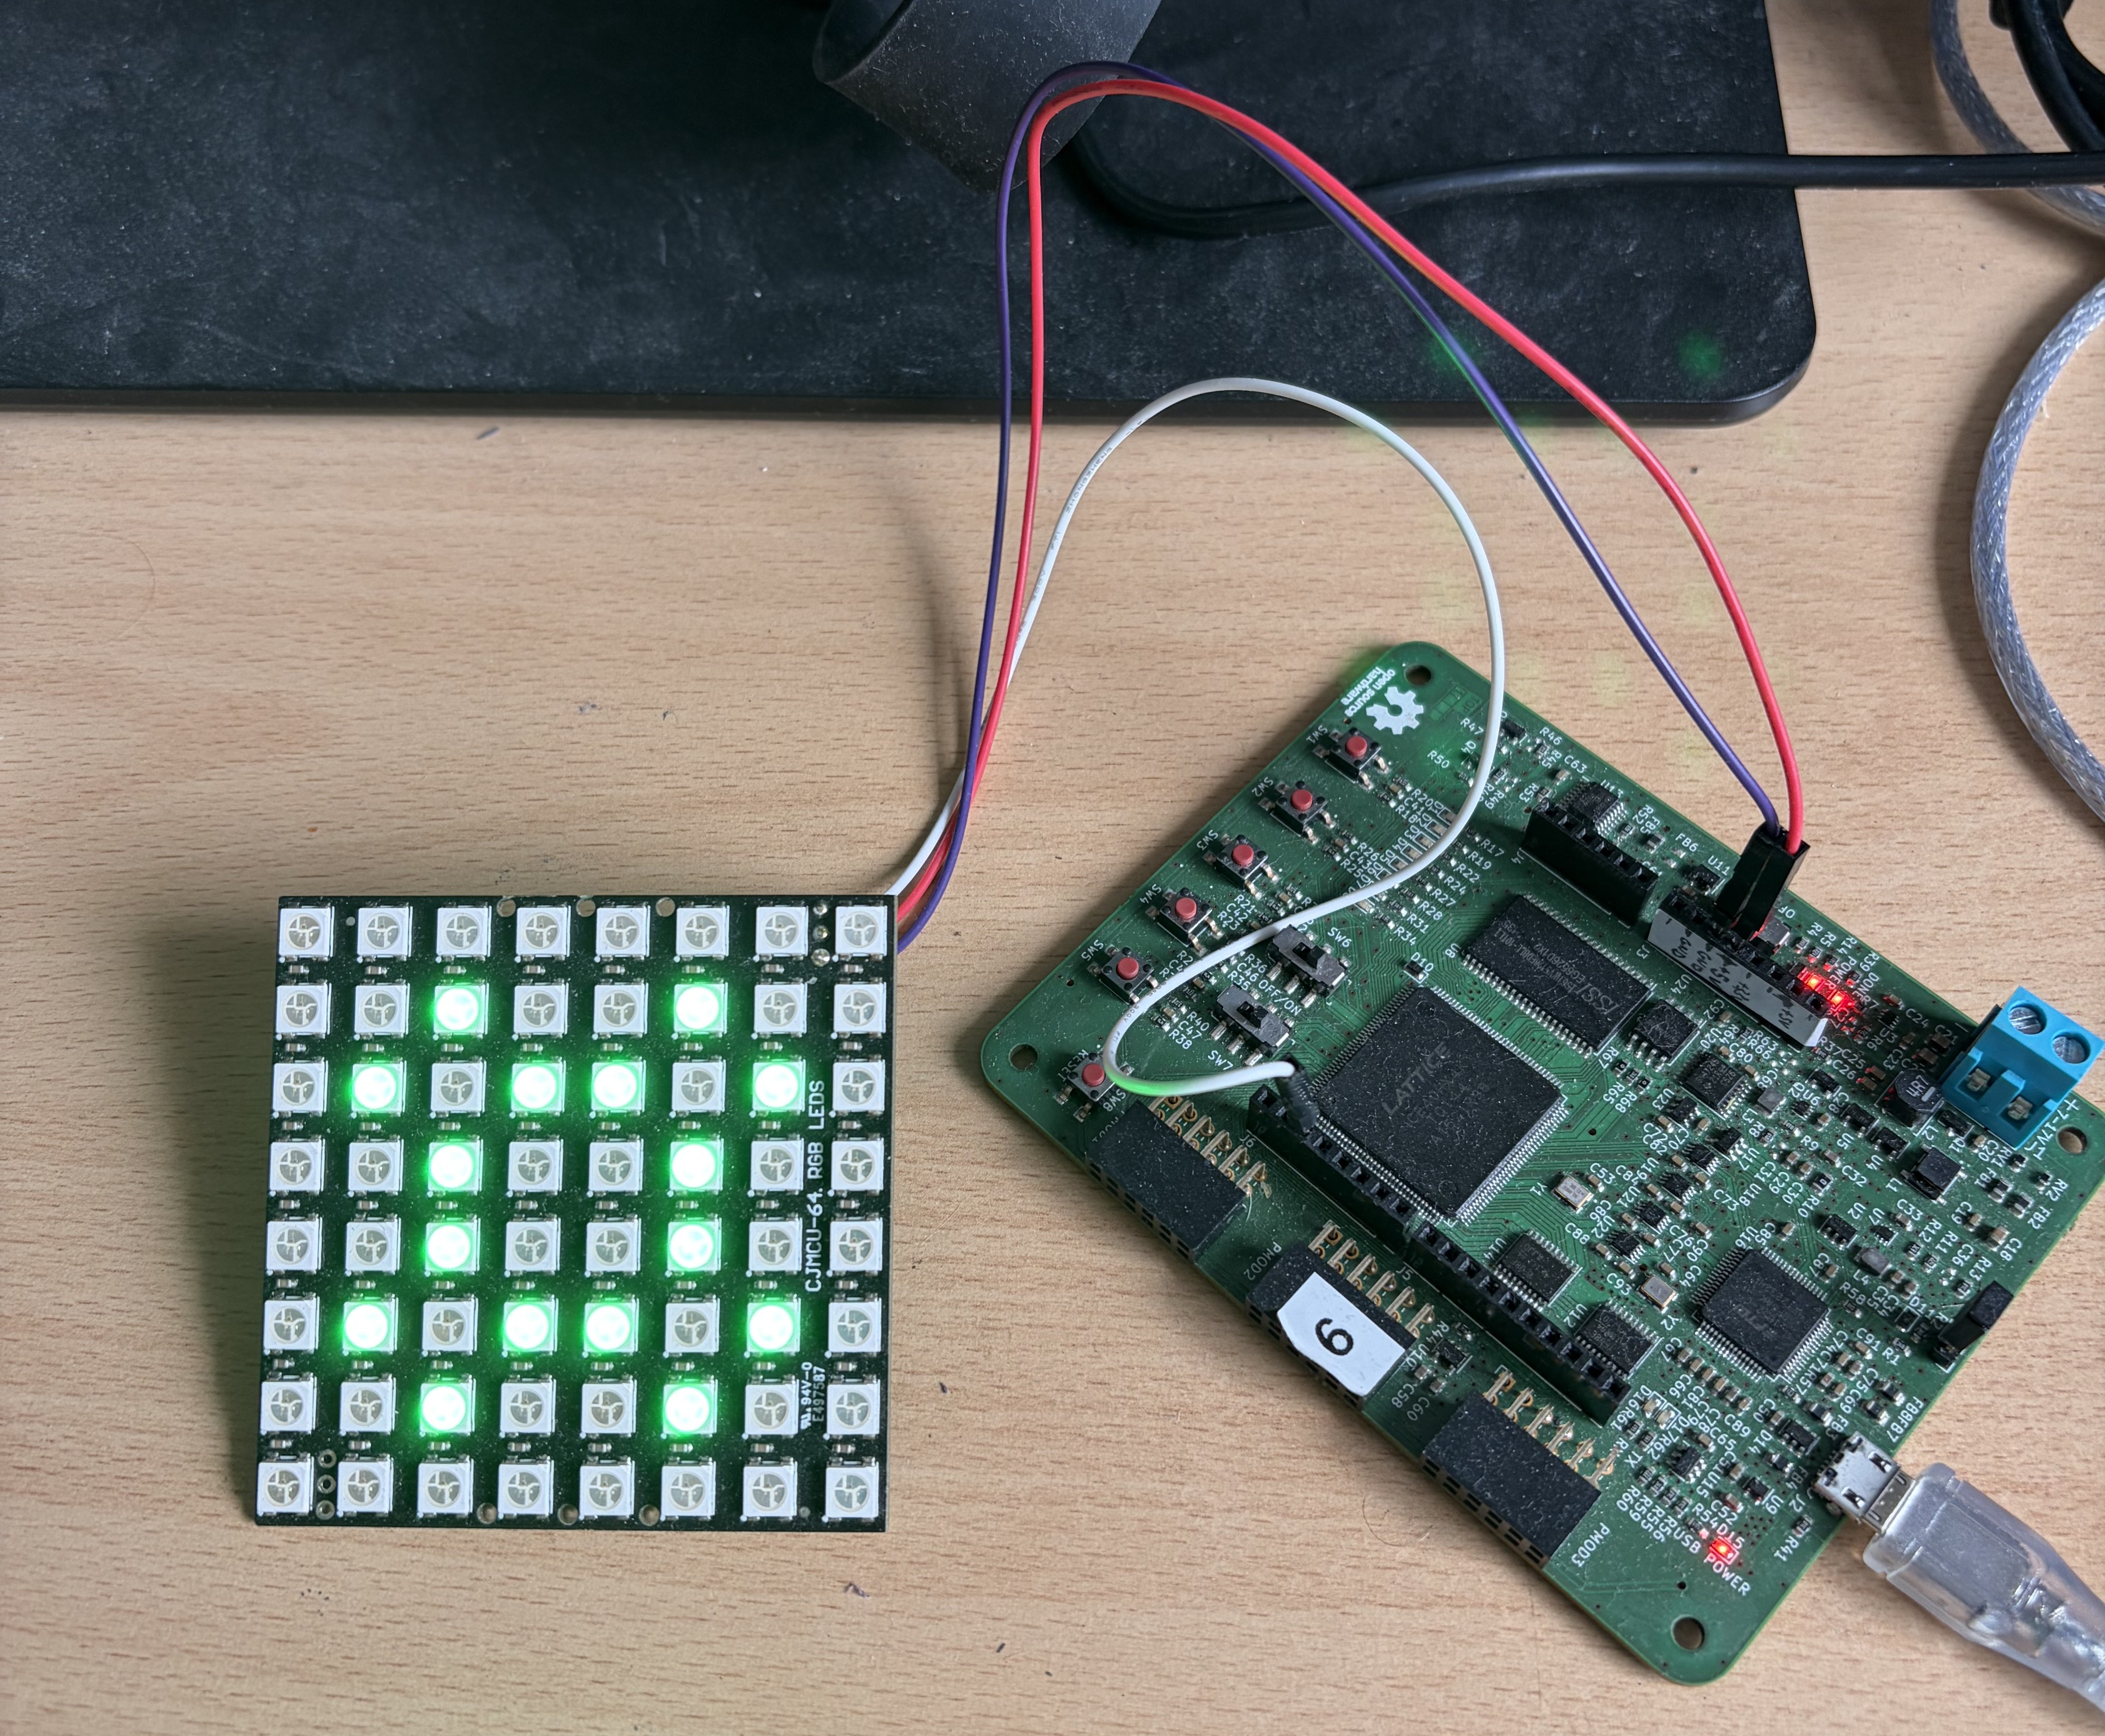
\includegraphics[width=\textwidth, angle=0]{A10_Abgabe/res/octagon_4.jpeg}
  \caption{Simulation des Octagon: Vierte Generation}
  \label{fig:octagon_4}
\end{figure}

\begin{figure}[H]
  \centering
  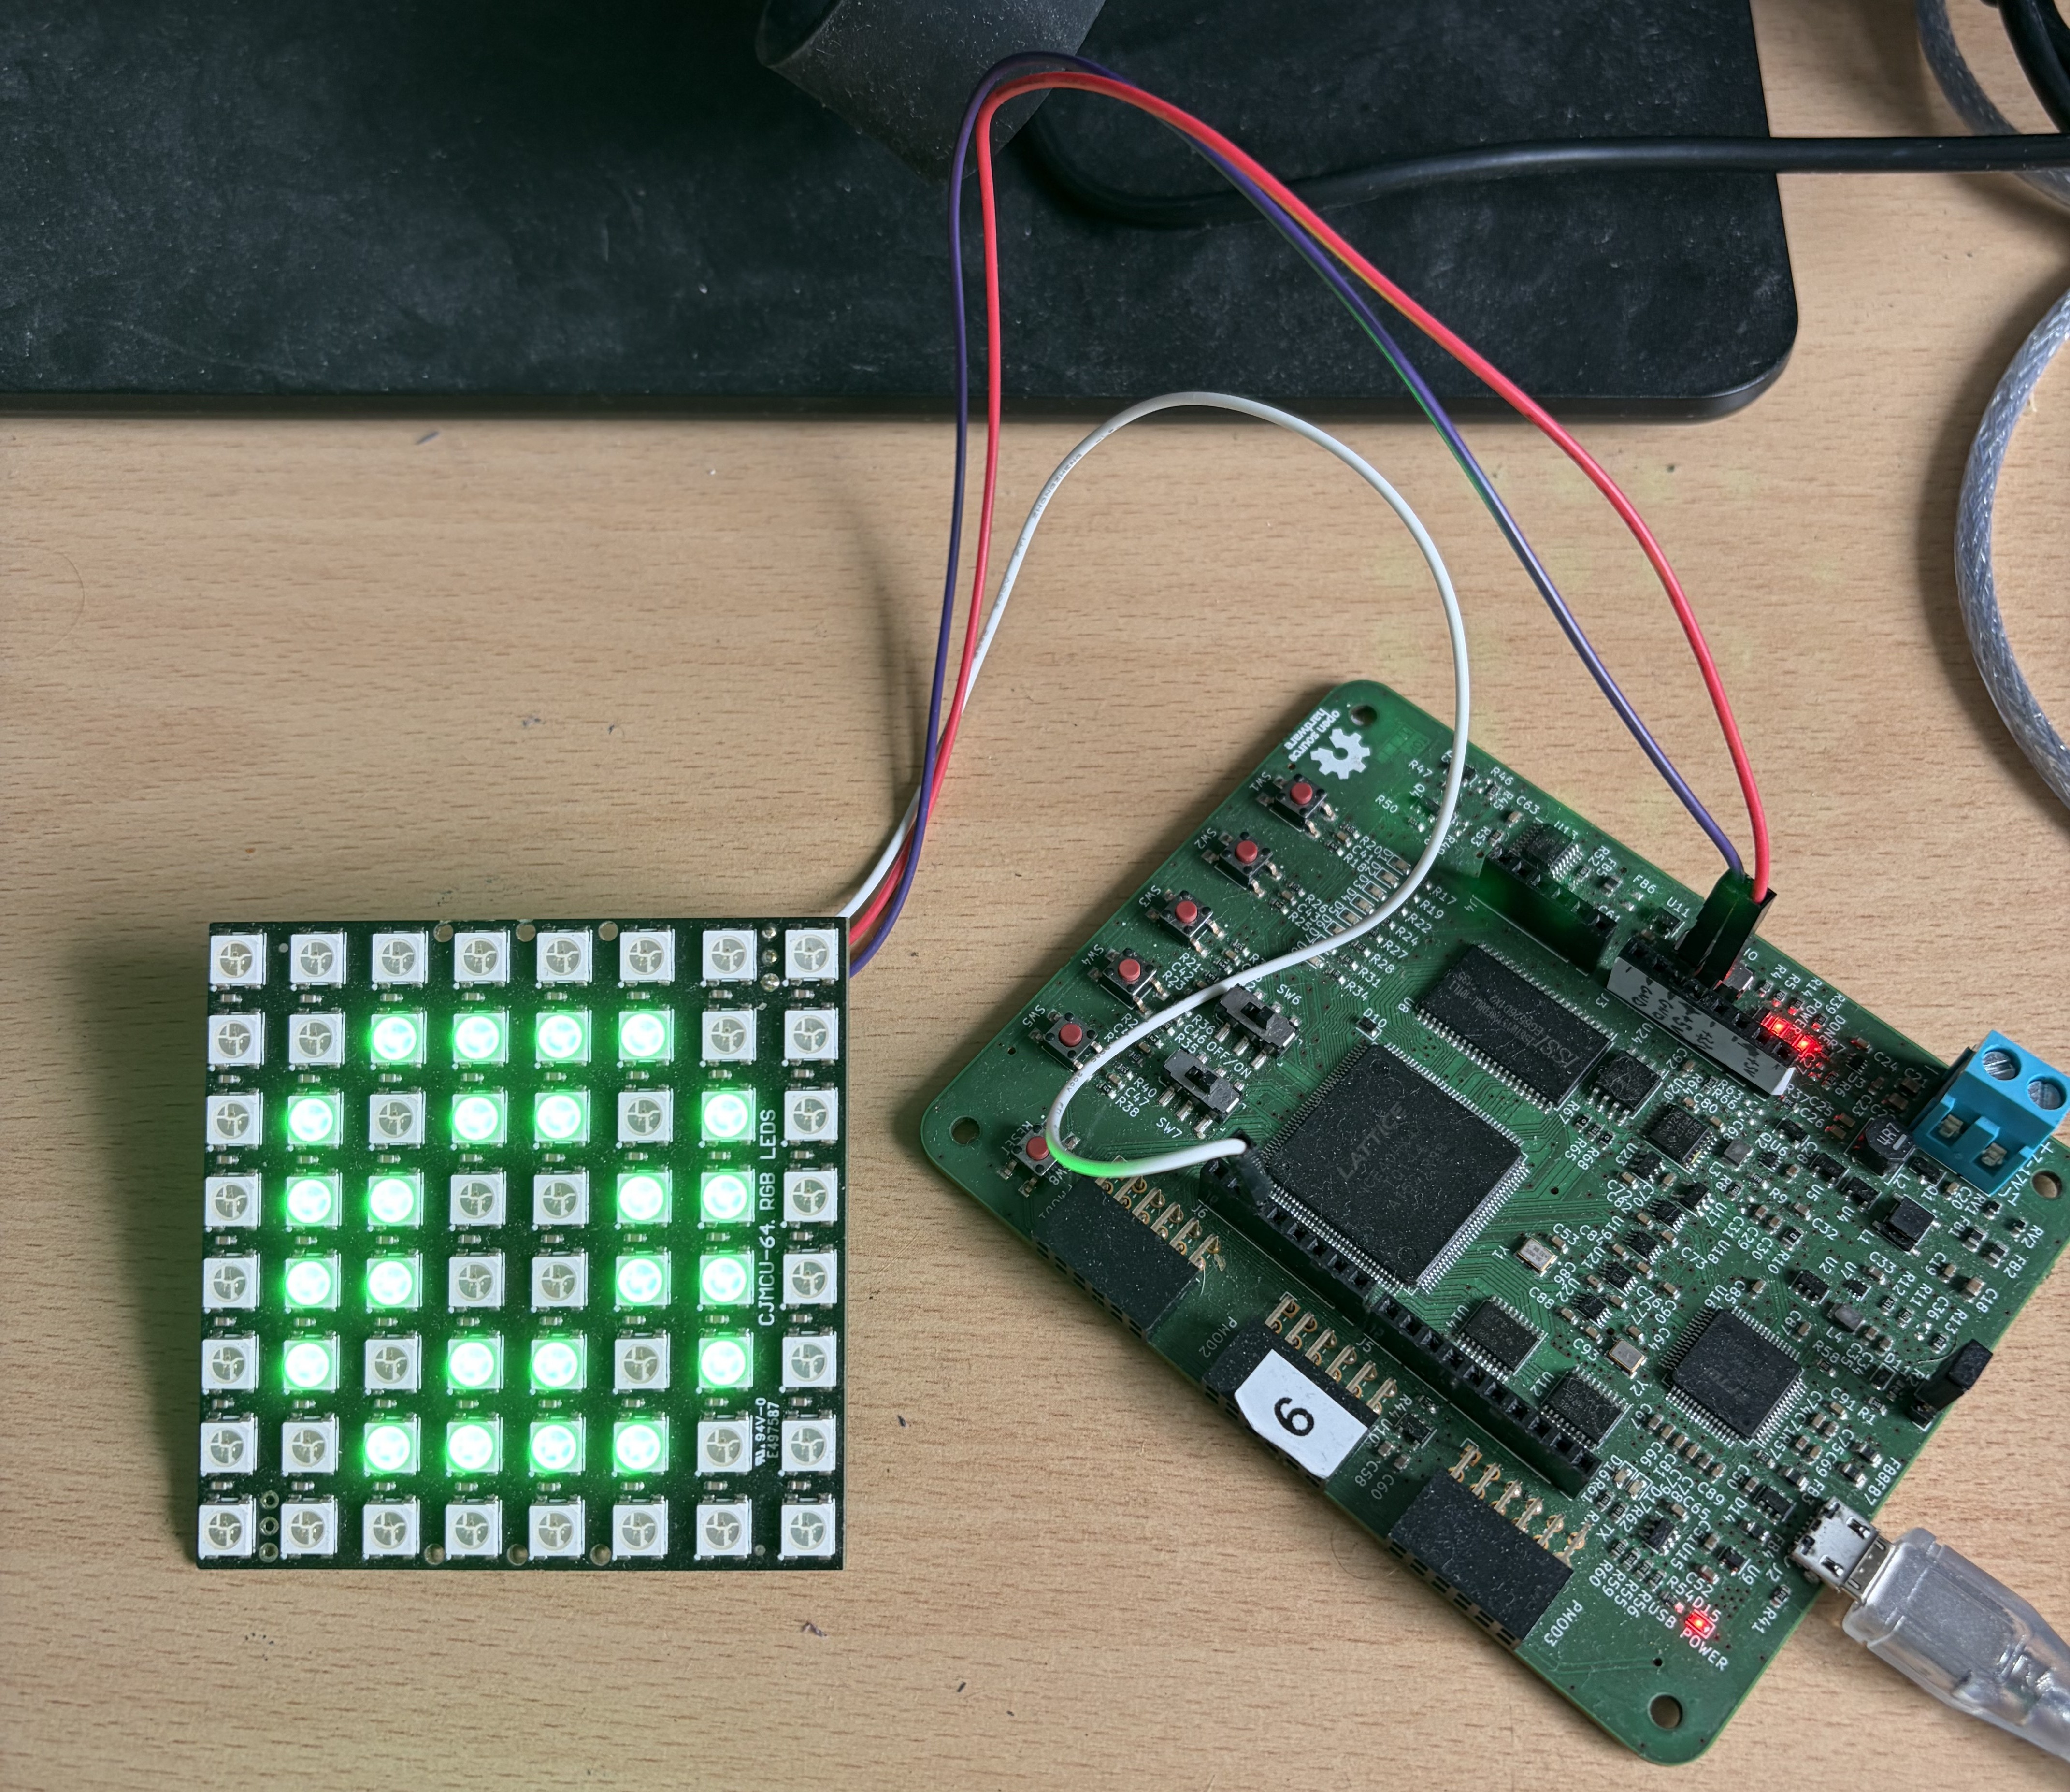
\includegraphics[width=\textwidth, angle=0]{A10_Abgabe/res/octagon_5.jpeg}
  \caption{Simulation des Octagon: Fünfte Generation}
  \label{fig:octagon_5}
\end{figure}

\subsection{Implementation des Pulsars}

Die Funktionsfähigkeit des Pulsars wurde ebenfalls überprüft. Dies ist in den
folgenden Abbildungen dargestellt. Hier ist die korrekte Funktionalität der
Nachbarzellenlogik zu erkennen, da der Pulsar ein GOL-Muster ist, welches mehr
als 8x8 Felder benötigt.

\begin{figure}[H]
  \centering
  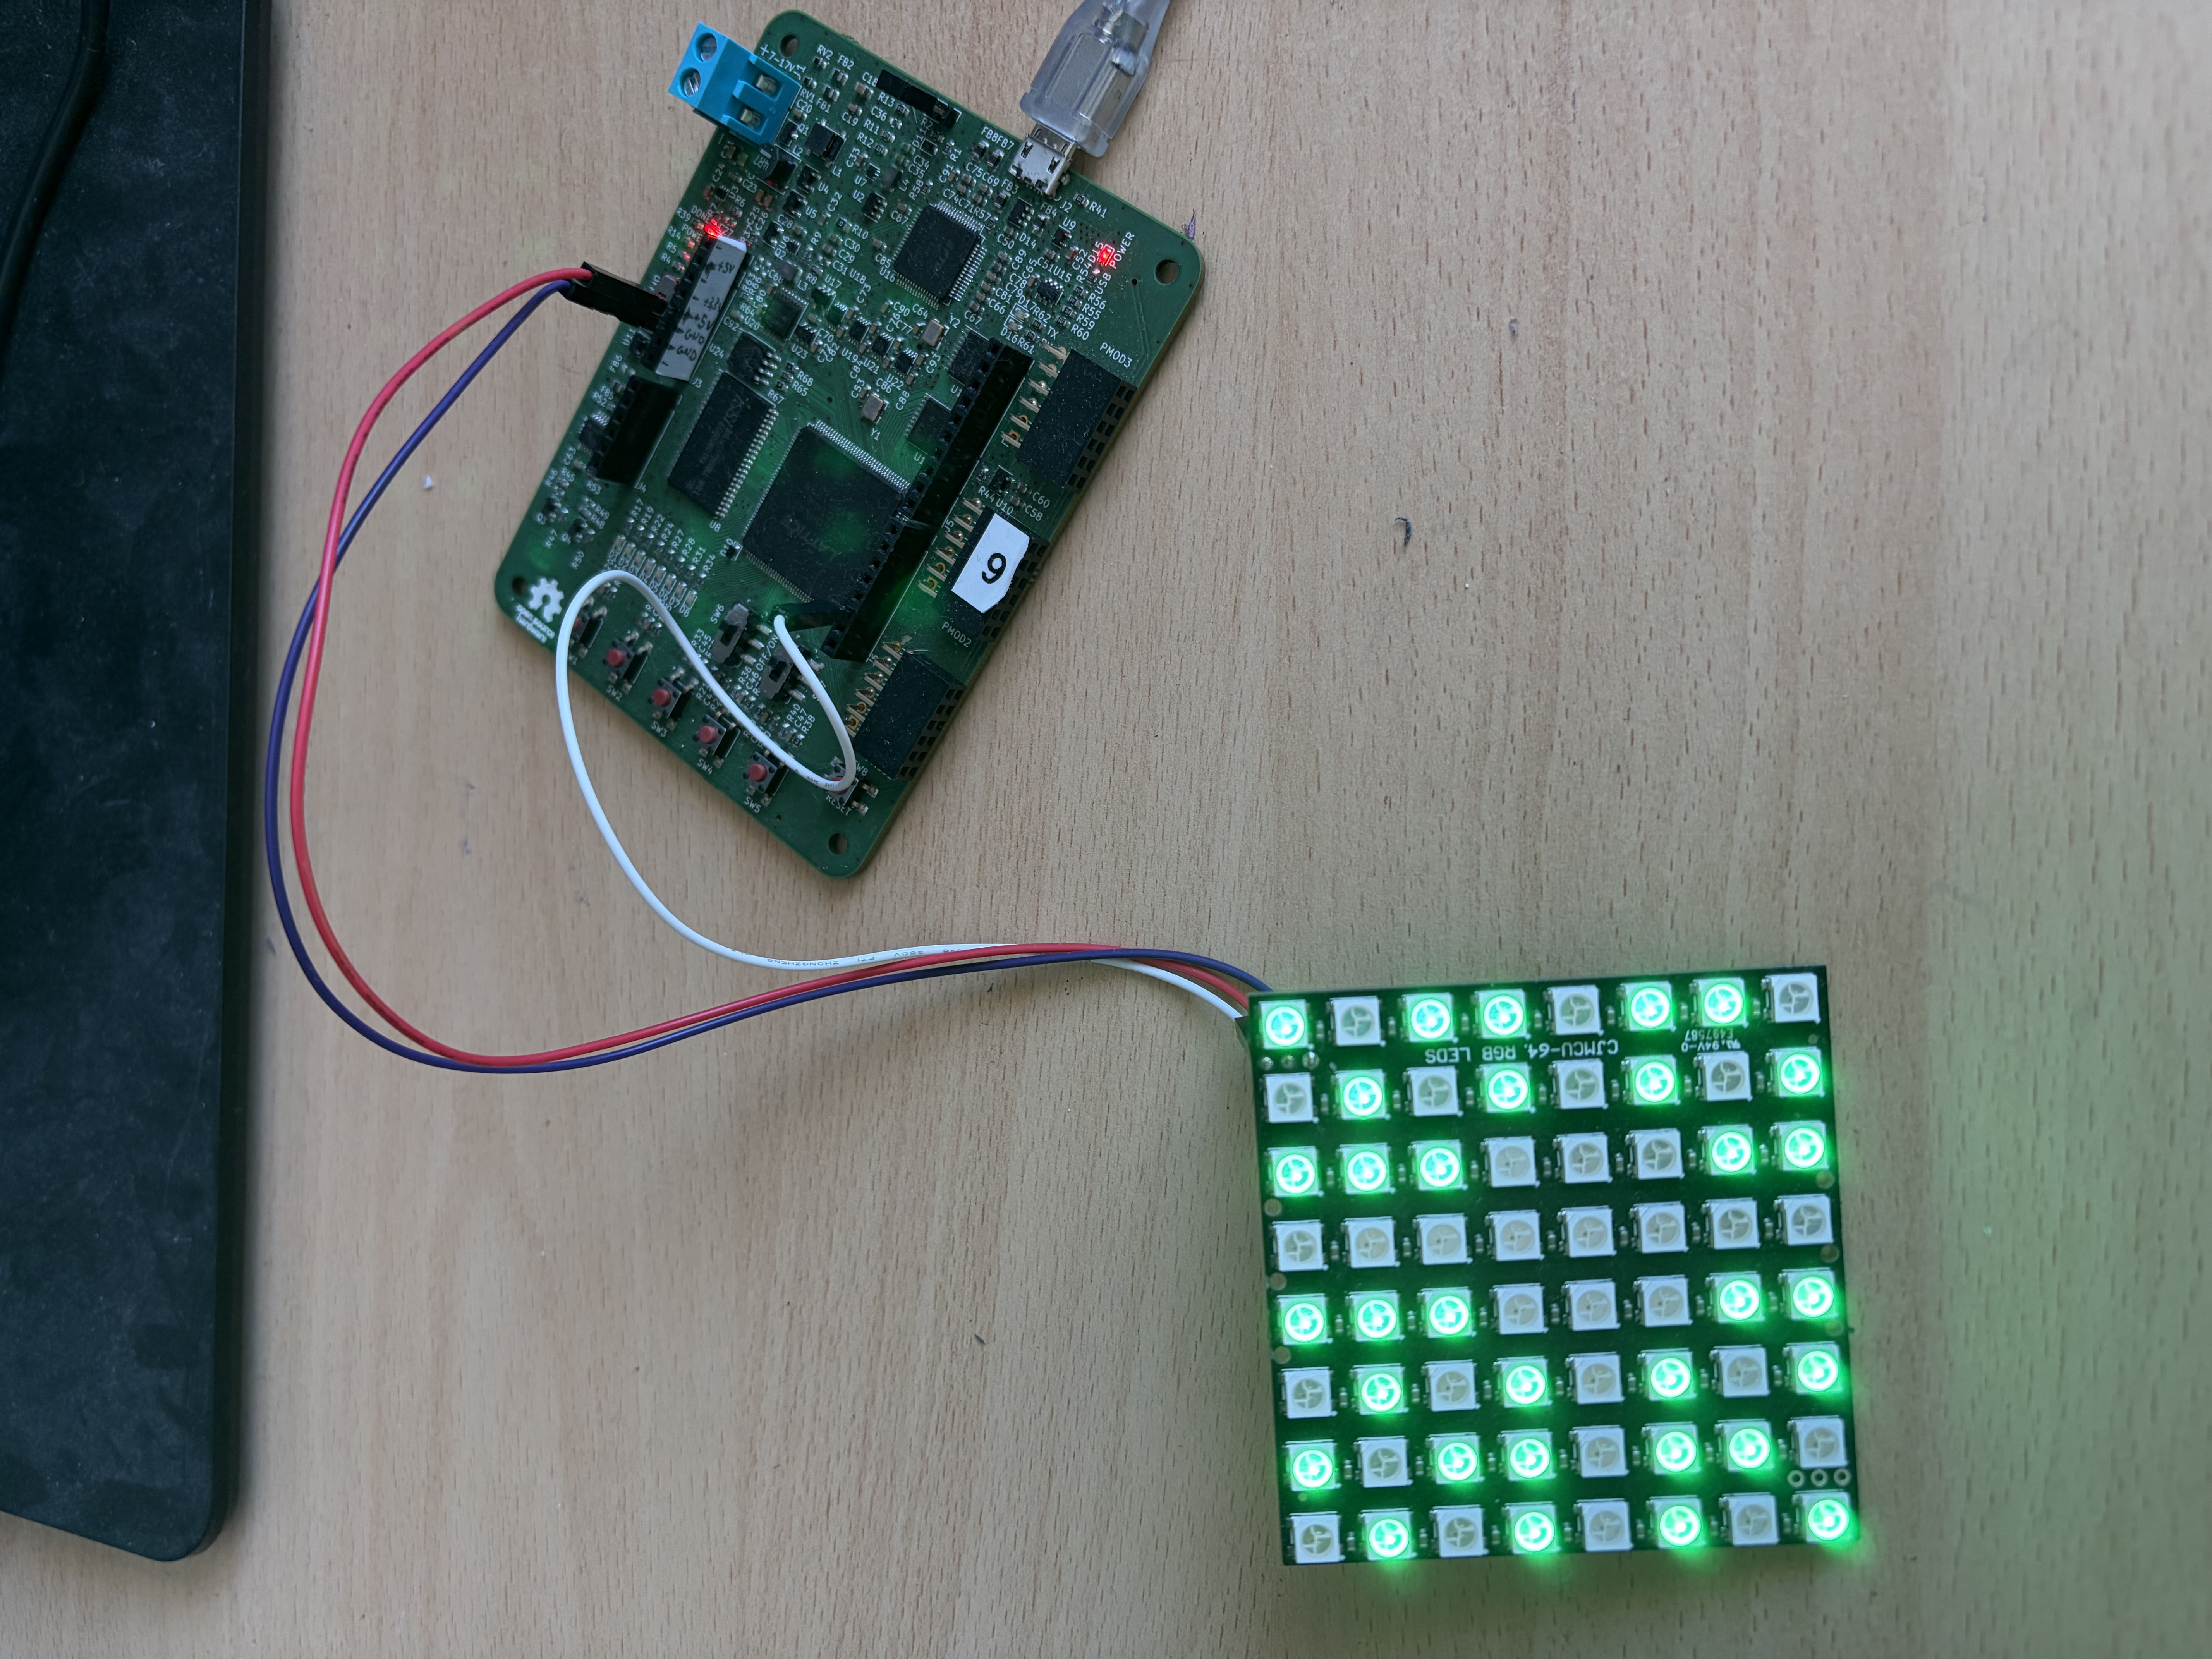
\includegraphics[width=\textwidth, angle=0]{A10_Abgabe/res/pulsar_1.jpeg}
  \caption{Simulation des Pulsars: Erste Generation}
  \label{fig:pulsar_1}
\end{figure}

\begin{figure}[H]
  \centering
  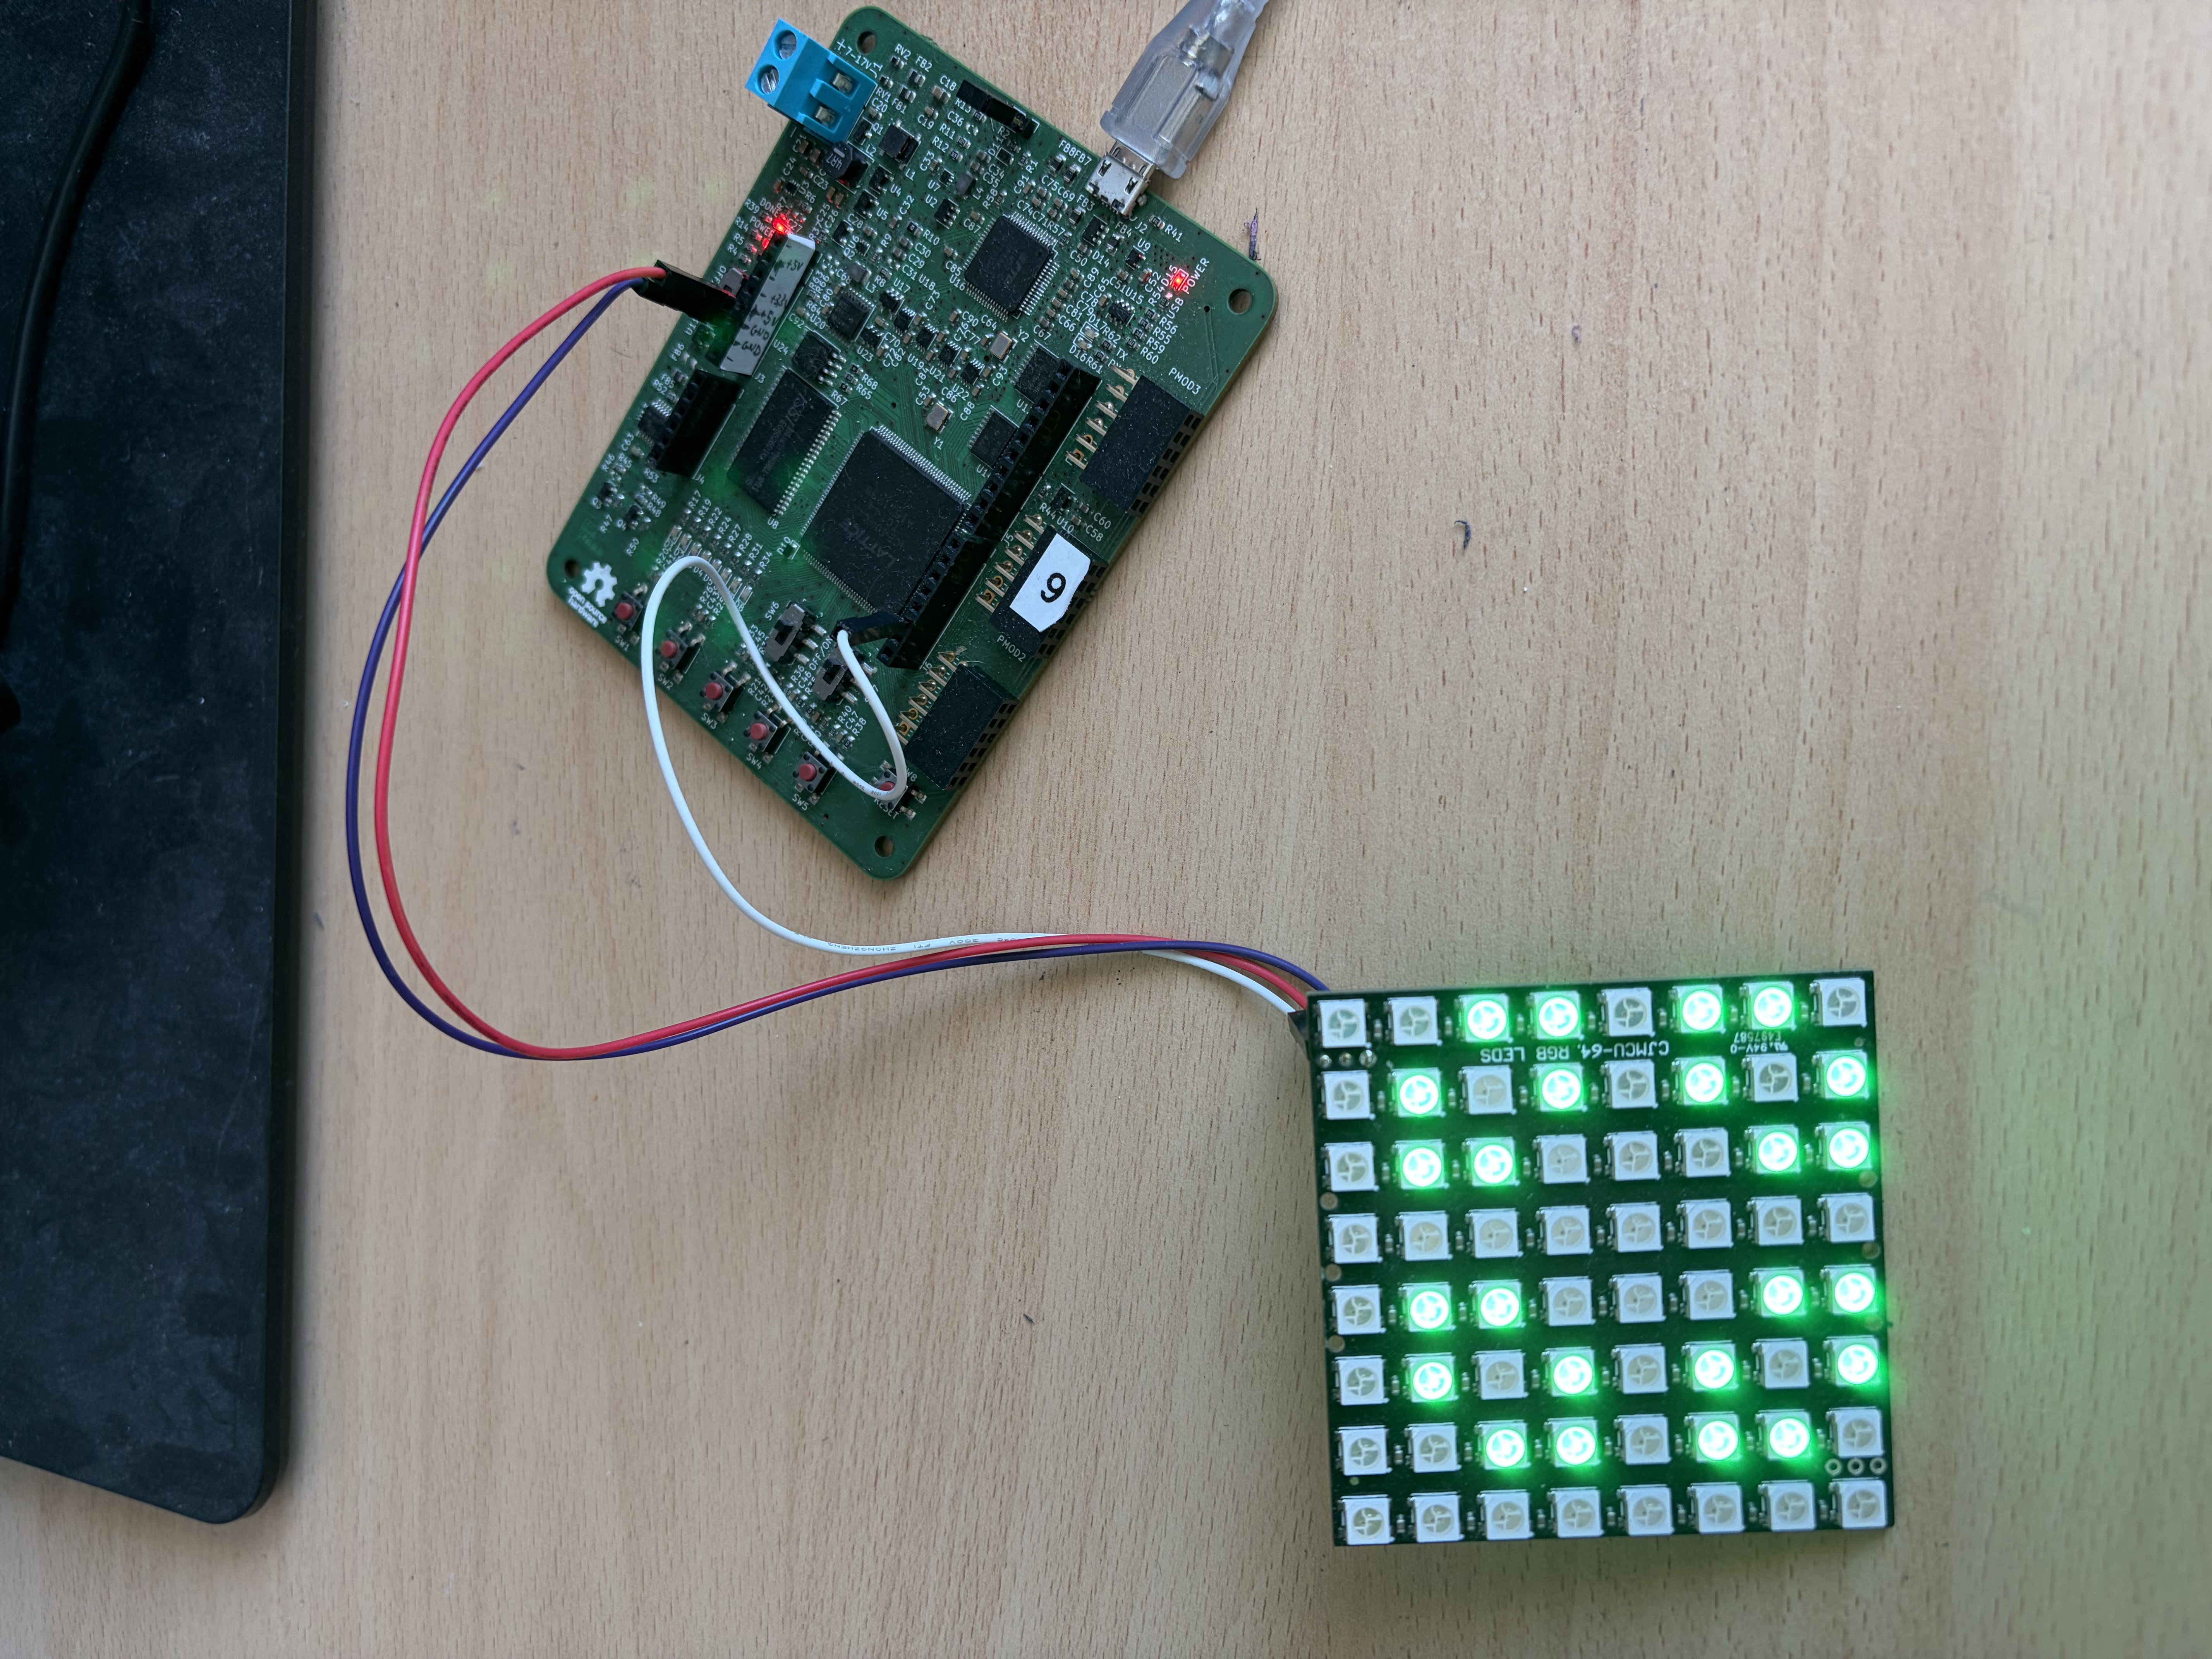
\includegraphics[width=\textwidth, angle=0]{A10_Abgabe/res/pulsar_2.jpeg}
  \caption{Simulation des Pulsars: Zweite Generation}
  \label{fig:pulsar_2}
\end{figure}

\begin{figure}[H]
  \centering
  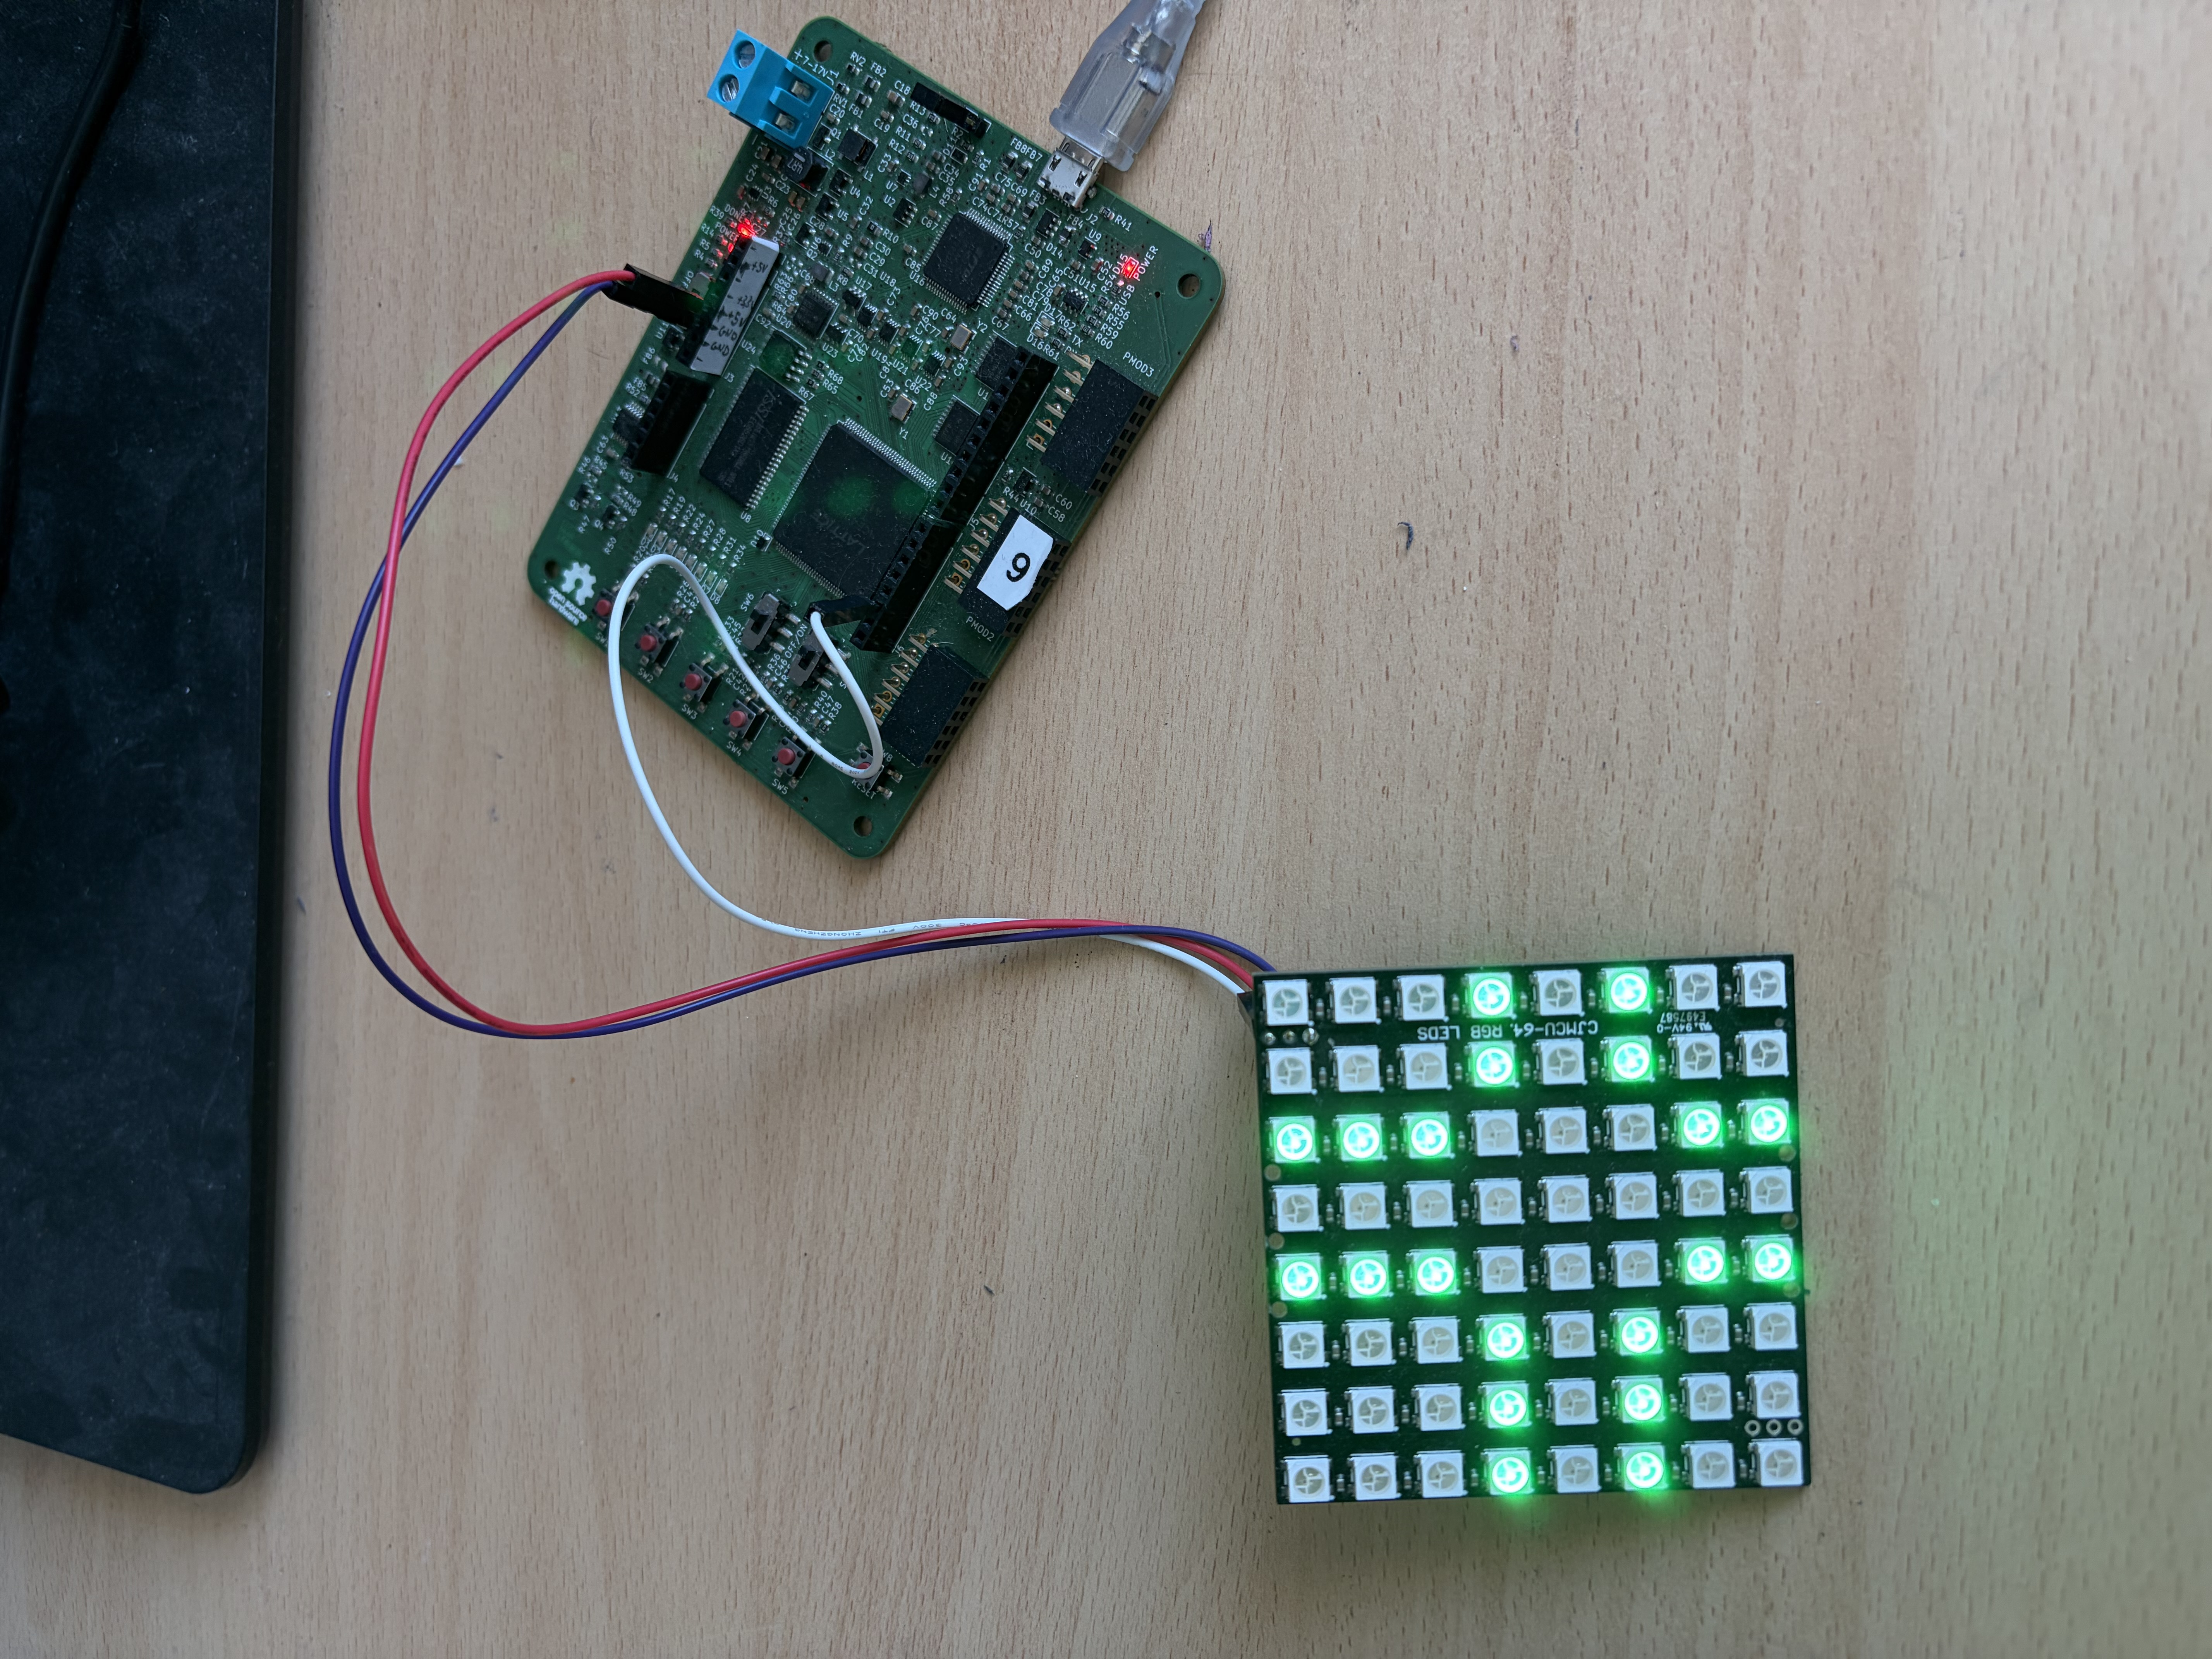
\includegraphics[width=\textwidth, angle=0]{A10_Abgabe/res/pulsar_3.jpeg}
  \caption{Simulation des Pulsars: Dritte Generation}
  \label{fig:pulsar_3}
\end{figure}

\subsection{Ausblick}

Um die Matrizen miteinander zu verbinden, muss die Kommunikation vollständig
implementiert werden. Dazu muss eine Schnittstelle mittels UART zu einem
Rechner implementiert werden, sodass Anweisungen an den Slave, in diesem Fall
an die LED-Matrix, gesendet werden können.

\subsection{Anhang}

main.c:
\inputminted[linenos,fontsize=\footnotesize]{c}{A10_Abgabe/iceduino_setup_gol/sw/programs/iceduino_game_of_life/main.c}
game\_of\_life.c:
\inputminted[linenos,fontsize=\footnotesize]{c}{A10_Abgabe/iceduino_setup_gol/sw/lib/source/game_of_life.c}
game\_of\_life.h:
\inputminted[linenos,fontsize=\footnotesize]{c}{A10_Abgabe/iceduino_setup_gol/sw/lib/include/game_of_life.h}
